
%  ========== PREAMBLE ==========

\documentclass[11pt]{article}

% -= Packages =-

\usepackage[top=1in,bottom=1in,left=1in,right=1in,paper=a4paper]{geometry}
\usepackage{graphicx,float}
\usepackage{hyperref}
\usepackage{tocloft}
\usepackage[immediate]{silence}
\WarningFilter[temp]{latex}{Command} % silence the warning
\usepackage{sectsty}
\DeactivateWarningFilters[temp] % So nothing unrelated gets silenced
\usepackage[most]{tcolorbox}
\usepackage{textcomp}
\usepackage{amsmath,amsfonts,amssymb,amsthm,mathtools,gensymb}
\usepackage{hyperref}
\usepackage{tikz}
\usepackage{titling}
\usepackage{lipsum}
\usepackage{mathtools}
\usepackage{enumitem}
\usepackage[utf8]{inputenc}
\usepackage[titletoc,title]{appendix}
\usepackage{xcolor}
\usepackage[twoside]{fancyhdr}
\usepackage[parfill]{parskip}
\usepackage{multicol}
\usepackage{pgfplots}
\pgfplotsset{compat=1.15}
\usepackage{mathrsfs}
\usetikzlibrary{arrows}
\usepackage{fontawesome5}
\usepackage{titlesec}

\usetikzlibrary{arrows.meta, decorations.pathreplacing,calc}

\makeatletter % disable the runtime redefinitions
\let\SS@makeulinesect\relax
\let\SS@makeulinepartchap\relax
\makeatother


% -= Settings =-

\pagestyle{fancy}
\allsectionsfont{\bfseries\sffamily}

\graphicspath{ {./images/} }

\hypersetup{
    colorlinks,
    citecolor=black,
    filecolor=black,
    linkcolor=purple,
    urlcolor=blue
}


\renewcommand{\baselinestretch}{1.5}
\newcommand{\qedblack}{$\hfill\blacksquare$}

\newcommand{\divides}{\mid}
\newcommand{\notdivides}{\nmid}

\DeclareMathOperator{\ord}{ord}

\DeclarePairedDelimiter\abs{\lvert}{\rvert}%
\DeclarePairedDelimiter\norm{\lVert}{\rVert}%

\renewcommand{\footrulewidth}{0.45pt}
\renewcommand{\headrulewidth}{0.45pt}
\definecolor{bbe}{HTML}{000000}
\definecolor{headerbg}{RGB}{0, 0, 0} 
\definecolor{headertext}{RGB}{255, 250, 240}
\definecolor{mahdarkblue}{HTML}{1e3f66}
\definecolor{mahdarknavy}{HTML}{254a6d}
\definecolor{mahnavy}{HTML}{2e5984}
\definecolor{mahblue}{HTML}{528aae}
\definecolor{mahlightblue}{HTML}{73a5c6}
\definecolor{mahsky}{HTML}{91bad6}
\definecolor{mahturquoise}{HTML}{5f8998}
\setlength{\headheight}{21pt}


% -= Theorem Environments =-

\newtcolorbox[auto counter,number within=section,number format=\arabic]{definition}[1][]{
            colback=mahdarkblue!10!white,enhanced,
            title={\textbf{\faBook\ \ Định nghĩa~\thetcbcounter}},
            attach boxed title to top left={xshift=-4mm},
            boxrule=0pt,
            after skip=1cm,before skip=1cm,right skip=0cm,
            breakable,fonttitle=\sffamily,
            toprule=0pt,bottomrule=0pt,rightrule=0pt,leftrule=4pt,
            arc=0mm,
            skin=enhancedlast jigsaw,
            sharp corners,
            colframe=mahdarkblue,colbacktitle=mahdarkblue!90!white,
            boxed title style={
                frame code={
                    \fill[mahdarkblue!90!white](frame.south west)--(frame.north west)--(frame.north east)--([xshift=3mm]frame.east)--(frame.south east)--cycle;
                    \draw[line width=1mm,mahdarkblue!90!white]([xshift=2mm]frame.north east)--([xshift=5mm]frame.east)--([xshift=2mm]frame.south east);
                    \draw[line width=1mm,mahdarkblue!90!white]([xshift=5mm]frame.north east)--([xshift=8mm]frame.east)--([xshift=5mm]frame.south east);
                    \fill[mahdarkblue!80!white](frame.south west)--+(4mm,-2mm)--+(4mm,2mm)--cycle;
                }
            }
}

\newtcolorbox[auto counter,number within=section,number format=\arabic]{theorem}[1][]{
            colback=mahdarknavy!10!white,enhanced,
            title={\textbf{\faPen\ \ Định lí~\thetcbcounter}},
            attach boxed title to top left={xshift=-4mm},
            boxrule=0pt,
            after skip=1cm,before skip=1cm,right skip=0cm,
            breakable,fonttitle=\sffamily,
            toprule=0pt,bottomrule=0pt,rightrule=0pt,leftrule=4pt,
            arc=0mm,
            skin=enhancedlast jigsaw,
            sharp corners,
            colframe=mahdarknavy,colbacktitle=mahdarknavy!90!white,
            boxed title style={
                frame code={
                    \fill[mahdarknavy!90!white](frame.south west)--(frame.north west)--(frame.north east)--([xshift=3mm]frame.east)--(frame.south east)--cycle;
                    \draw[line width=1mm,mahdarknavy!90!white]([xshift=2mm]frame.north east)--([xshift=5mm]frame.east)--([xshift=2mm]frame.south east);
                    \draw[line width=1mm,mahdarknavy!90!white]([xshift=5mm]frame.north east)--([xshift=8mm]frame.east)--([xshift=5mm]frame.south east);
                    \fill[mahdarknavy!80!white](frame.south west)--+(4mm,-2mm)--+(4mm,2mm)--cycle;
                }
            }
}

\newtcolorbox[auto counter,number within=section,number format=\arabic]{property}[1][]{
            colback=mahnavy!10!white,enhanced,
            title={\textbf{\faBookmark\ \ Tính chất~\thetcbcounter}},
            attach boxed title to top left={xshift=-4mm},
            boxrule=0pt,
            after skip=1cm,before skip=1cm,right skip=0cm,
            breakable,fonttitle=\sffamily,
            toprule=0pt,bottomrule=0pt,rightrule=0pt,leftrule=4pt,
            arc=0mm,
            skin=enhancedlast jigsaw,
            sharp corners,
            colframe=mahnavy,colbacktitle=mahnavy!90!white,
            boxed title style={
                frame code={
                    \fill[mahnavy!90!white](frame.south west)--(frame.north west)--(frame.north east)--([xshift=3mm]frame.east)--(frame.south east)--cycle;
                    \draw[line width=1mm,mahnavy!90!white]([xshift=2mm]frame.north east)--([xshift=5mm]frame.east)--([xshift=2mm]frame.south east);
                    \draw[line width=1mm,mahnavy!90!white]([xshift=5mm]frame.north east)--([xshift=8mm]frame.east)--([xshift=5mm]frame.south east);
                    \fill[mahnavy!80!white](frame.south west)--+(4mm,-2mm)--+(4mm,2mm)--cycle;
                }
            }
}

\newtcolorbox[auto counter,number format=\arabic]{problem}[1][]{
            colback=mahblue!10!white,enhanced,
            title={\textbf{\faFile*\ \ Problem~\thetcbcounter}},
            attach boxed title to top left={xshift=-4mm},
            boxrule=0pt,
            after skip=1cm,before skip=1cm,right skip=0cm,
            breakable,fonttitle=\sffamily,
            toprule=0pt,bottomrule=0pt,rightrule=0pt,leftrule=4pt,
            arc=0mm,
            skin=enhancedlast jigsaw,
            sharp corners,
            colframe=mahblue,colbacktitle=mahblue!90!white,
            boxed title style={
                frame code={
                    \fill[mahblue!90!white](frame.south west)--(frame.north west)--(frame.north east)--([xshift=3mm]frame.east)--(frame.south east)--cycle;
                    \draw[line width=1mm,mahblue!90!white]([xshift=2mm]frame.north east)--([xshift=5mm]frame.east)--([xshift=2mm]frame.south east);
                    \draw[line width=1mm,mahblue!90!white]([xshift=5mm]frame.north east)--([xshift=8mm]frame.east)--([xshift=5mm]frame.south east);
                    \fill[mahblue!80!white](frame.south west)--+(4mm,-2mm)--+(4mm,2mm)--cycle;
                }
            }
}

\newtcolorbox[auto counter,number within=section,number format=\arabic]{problemme}[1][]{
            colback=mahblue!10!white,enhanced,
            title={\textbf{\faFile*\ \ Problem statement}},
            attach boxed title to top left={xshift=-4mm},
            boxrule=0pt,
            after skip=1cm,before skip=1cm,right skip=0cm,
            breakable,fonttitle=\sffamily,
            toprule=0pt,bottomrule=0pt,rightrule=0pt,leftrule=4pt,
            arc=0mm,
            skin=enhancedlast jigsaw,
            sharp corners,
            colframe=mahblue,colbacktitle=mahblue!90!white,
            boxed title style={
                frame code={
                    \fill[mahblue!90!white](frame.south west)--(frame.north west)--(frame.north east)--([xshift=3mm]frame.east)--(frame.south east)--cycle;
                    \draw[line width=1mm,mahblue!90!white]([xshift=2mm]frame.north east)--([xshift=5mm]frame.east)--([xshift=2mm]frame.south east);
                    \draw[line width=1mm,mahblue!90!white]([xshift=5mm]frame.north east)--([xshift=8mm]frame.east)--([xshift=5mm]frame.south east);
                    \fill[mahblue!80!white](frame.south west)--+(4mm,-2mm)--+(4mm,2mm)--cycle;
                }
            }
}

\newtcolorbox[auto counter,number format=\arabic]{exproblem}[1][]{
            colback=mahblue!10!white,enhanced,
            title={\textbf{\faFile*\ \ Ví dụ~\thetcbcounter}},
            attach boxed title to top left={xshift=-4mm},
            boxrule=0pt,
            after skip=1cm,before skip=1cm,right skip=0cm,
            breakable,fonttitle=\sffamily,
            toprule=0pt,bottomrule=0pt,rightrule=0pt,leftrule=4pt,
            arc=0mm,
            skin=enhancedlast jigsaw,
            sharp corners,
            colframe=mahblue,colbacktitle=mahblue!90!white,
            boxed title style={
                frame code={
                    \fill[mahblue!90!white](frame.south west)--(frame.north west)--(frame.north east)--([xshift=3mm]frame.east)--(frame.south east)--cycle;
                    \draw[line width=1mm,mahblue!90!white]([xshift=2mm]frame.north east)--([xshift=5mm]frame.east)--([xshift=2mm]frame.south east);
                    \draw[line width=1mm,mahblue!90!white]([xshift=5mm]frame.north east)--([xshift=8mm]frame.east)--([xshift=5mm]frame.south east);
                    \fill[mahblue!80!white](frame.south west)--+(4mm,-2mm)--+(4mm,2mm)--cycle;
                }
            }
}

\newtcolorbox[auto counter,number within=section,number format=\arabic]{corollary}[1][]{
            colback=mahlightblue!10!white,enhanced,
            title={\textbf{\faHandPointRight[regular] \ \ Hệ quả \thetcbcounter}},
            boxrule=0pt,
	    frame hidden,
            breakable,fonttitle=\sffamily,
            arc=0mm,
            sharp corners,
            detach title,
            before upper = \tcbtitle\par\smallskip,
            colframe=mahlightblue,coltitle=mahlightblue!85!black,
            borderline west = {1mm}{0pt}{mahlightblue!85!black},
            segmentation style={solid, mahlightblue!85!black}
}

\newtcolorbox[auto counter,number format=\arabic]{lemma}[1][]{
            colback=mahlightblue!10!white,enhanced,
            title={\textbf{\faBook \ \ Bổ đề}},
            boxrule=0pt,
	    frame hidden,
            breakable,fonttitle=\sffamily,
            arc=0mm,
            sharp corners,
            detach title,
            before upper = \tcbtitle\par\smallskip,
            colframe=mahlightblue,coltitle=mahlightblue!85!black,
            borderline west = {1mm}{0pt}{mahlightblue!85!black},
            segmentation style={solid, mahlightblue!85!black}
}

\newtcolorbox[auto counter,number format=\arabic]{claim}[1][]{
            colback=mahturquoise!10!white,enhanced,
            title={\textbf{\faExclamation \ \ Claim --- \ }},
            boxrule=0pt,
	    frame hidden,
            breakable,fonttitle=\sffamily,
            arc=0mm,
            sharp corners,
            detach title,
            before upper = \tcbtitle,
            colframe=mahturquoise,coltitle=mahturquoise!85!black,
            borderline west = {1mm}{0pt}{mahturquoise!85!black},
            segmentation style={solid, mahturquoise!85!black}
}

\newtcolorbox[auto counter,number format=\arabic]{remark}[1][]{
            colback=mahsky!10!white,enhanced,
            title={\textbf{\faExclamation \ \ Remark --- \ }},
            boxrule=0pt,
	    frame hidden,
            breakable,fonttitle=\sffamily,
            arc=0mm,
            sharp corners,
            detach title,
            before upper = \tcbtitle,
            colframe=mahsky,coltitle=mahsky!85!black,
            borderline west = {1mm}{0pt}{mahsky!85!black},
            segmentation style={solid, mahsky!85!black}
}

\newtcolorbox[auto counter,number format=\arabic]{motivation}[1][]{
            colback=mahlightblue!10!white,enhanced,
            title={\textbf{\faQuestion \ \ Motivation}},
            boxrule=0pt,
	    frame hidden,
            breakable,fonttitle=\sffamily,
            arc=0mm,
            sharp corners,
            detach title,
            before upper = \tcbtitle\par\smallskip,
            colframe=mahlightblue,coltitle=mahlightblue!85!black,
            borderline west = {1mm}{0pt}{mahlightblue!85!black},
            segmentation style={solid, mahlightblue!85!black}
}

\newenvironment{solution}[1][Solution]{%
  \proof[\normalfont \faPenNib \hspace{0.2cm} \ttfamily \scshape \large #1]%
}{\(\hfill \blacksquare\){\parfillskip0pt\par}}

\theoremstyle{definition}
\newtheorem{exercise}{Problem}

\newcommand{\boom}{\vspace{0.25cm}}


% -= Header + Title =-

% Header

\fancyhead[RO]{\footnotesize \thepage}
\fancyhead[RE]{\footnotesize \textsc{VMO 2013 Solution Notes}}
\fancyhead[LE]{\footnotesize \thepage}
\fancyhead[LO]{\footnotesize \scshape Mark Nguyen}
\fancyfoot{}

\renewcommand{\footrulewidth}{0pt}

% Section title

\makeatletter
\titleformat{\section}
  {\normalfont\Large\bfseries\sffamily}{\color{purple}\S\thesection}{1em}{}
\titleformat{\subsection}
  {\normalfont\large\bfseries\sffamily}{\color{purple}\S\thesubsection}{1em}{}
\titleformat{\subsubsection}
  {\normalfont\normalsize\bfseries\ttfamily}{\color{purple}\S\thesubsubsection}{1em}{}
\makeatother
  

\renewcommand{\cfttoctitlefont}{\hfill\bfseries\LARGE}
\renewcommand{\cftaftertoctitle}{\hfill\hspace{-1cm}}

\title{\textbf{\Huge VMO 2013 Solution Notes}}
\author{\LARGE \textsc{Mark Nguyen}}
\date{\sffamily\today}

\begin{document}

\maketitle

\begin{abstract}
    This document compiles my solutions and best attempts for the 2013 Vietnamese Mathematical Olympiad. While I originally considered writing in Vietnamese, I chose English to make it accessible to a wider audience and to refine my language skills. All content is authored and maintained by me. Comments and corrections are welcome.
\end{abstract}

\tableofcontents

\newpage

\section{Problems}

    \subsection*{Day 1}

        \begin{exercise}
            Solve the following system of equations over \(\mathbb{R}\)
            \[\begin{cases}
                \sqrt{\left(\sin x\right)^2 + \dfrac{1}{\left(\sin x\right)^2}} + \sqrt{\left(\cos y\right)^2 + \dfrac{1}{\left(\cos y\right)^2}} = \sqrt{\dfrac{20y}{x + y}} \\
                \sqrt{\left(\sin y\right)^2 + \dfrac{1}{\left(\sin y\right)^2}} + \sqrt{\left(\cos x\right)^2 + \dfrac{1}{\left(\cos x\right)^2}} = \sqrt{\dfrac{20x}{x + y}}
            \end{cases}.\]
        \end{exercise}
    
        \boom
    
        \begin{exercise}
            Define a sequence \((a_n)_{n=1}^{+\infty}\) as follows
            \[\begin{cases}
                a_1 = 1 \\
                a_{n+1} = 3 - \dfrac{a_n + 2}{2^{a_n}} 
            \end{cases}.\]
            Prove that the sequence \((a_n)\) has a finite limit and find this limit.
        \end{exercise}
    
        \boom
    
        \begin{exercise}
            Let \(ABC\) be a scalene triangle. The incircle \((I)\) of triangle \(ABC\) touches \(BC\), \(CA\), and \(AB\) at \(D\), \(E\), and \(F\) respectively. The line passing through \(E\) and perpendicular to \(BI\) intersects \((I)\) at \(K\) (\(K \neq B\)). The line passing through \(F\) and perpendicular to \(CI\) intersects \((I)\) at \(L\) (\(L \neq C\)). Let \(J\) be the midpoint of the segment \(KL\).
            \begin{enumerate}
                \item[(a)] Prove that \(D\), \(I\), \(J\) are collinear.
                \item[(b)] Suppose that the points \(B\) and \(C\) are fixed and \(A\) is a moving point such that \(\dfrac{AB}{AC} = k\) (where \(k \in \mathbb{R}^+\) is a given constant). The lines \(IE\) and \(IF\) intersect \((I)\) again at \(M\) and \(N\) respectively. The line \(MN\) intersects \(IB\) at \(P\) and intersects \(IC\) at \(Q\). Prove that the perpendicular bisector of the segment \(PQ\) passes through a fixed point.
            \end{enumerate}
        \end{exercise}
    
        \boom
    
        \begin{exercise}
            Several natural numbers are given on a line. At each step, we perform the transformation as follows: consider all adjacent pairs of numbers on the line, from left to right, write in the middle of each pair with its sum. After 2013 such steps, how many times the number 2013 appears on the line if the initial numbers are
            \begin{enumerate}
                \item[(a)] 1 and 1000?
                \item[(b)] the first 1000 natural numbers on the increasing order from left to right?
            \end{enumerate}
        \end{exercise}

    \newpage
    
    \subsection*{Day 2}

        \begin{exercise}
            Find all functions \(f: \mathbb{R} \to \mathbb{R}\) satisfy \(f(0) = 0\), \(f(1) = 2013\), and
            \[(x - y)\left(f\left(\left(f(x)\right)^2\right) - f\left(\left(f(y)\right)^2\right)\right) = \left(f(x) - f(y)\right)\left(\left(f(x)\right)^2 - \left(f(y)\right)^2\right).\]
        \end{exercise}
    
        \boom
    
        \begin{exercise}
            Let \(ABC\) be an acute triangle with circumcircle \((O)\). \(D\) is a point on arc \(BC\) not containing \(A\). A moving line \(\ell\) passes through orthocenter \(H\) of triangle \(ABC\) and intersects the circumcircle of triangle \(ABH\) and triangle \(ACH\) at \(M\) and \(N\) respectively (\(M \neq H\), \(N \neq H\)).
            \begin{enumerate}
                \item[(a)] Determine the position of \(\ell\) such that the area of triangle \(AMN\) attains maximal value.
                \item[(b)] Denote \(d_1\) be the line passing through \(M\) and perpendicular to \(DB\), \(d_2\) be the line passing through \(N\) and perpendicular to \(DC\). Prove that intersection \(P\) of the lines \(d_1\) and \(d_2\) lies on a fixed circle.
            \end{enumerate}
        \end{exercise}
    
        \boom
    
        \begin{exercise}
            Find the number of ordered 6-tuples \((a,b,c,a',b',c')\) satisfy the following system of modular equations
            \[\begin{cases}
                ab + a'b' \equiv 1 \pmod{15} \\
                bc + b'c' \equiv 1 \pmod{15} \\
                ca + c'a' \equiv 1 \pmod{15} 
            \end{cases},\]
            of which \(a,b,c,a',b',c' \in \{0,1,2,\dots,14\}\).
        \end{exercise}

    \newpage

\section{Solutions}

    \subsection{Solutions for Day 1}

        \begin{problem}
            Solve the following system of equations over \(\mathbb{R}\)
            \[\begin{cases}
                \sqrt{\left(\sin x\right)^2 + \dfrac{1}{\left(\sin x\right)^2}} + \sqrt{\left(\cos y\right)^2 + \dfrac{1}{\left(\cos y\right)^2}} = \sqrt{\dfrac{20y}{x + y}} \\
                \sqrt{\left(\sin y\right)^2 + \dfrac{1}{\left(\sin y\right)^2}} + \sqrt{\left(\cos x\right)^2 + \dfrac{1}{\left(\cos x\right)^2}} = \sqrt{\dfrac{20x}{x + y}}
            \end{cases}.\]
        \end{problem}

        \begin{solution}
            The solutions are \((x,y) = \left(\dfrac{\pi}{4} + \dfrac{k\pi}{2}, \dfrac{\pi}{4} + \dfrac{k\pi}{2}\right)\), where \(k \in \mathbb{Z}\).\\
            Conversely, notice that \(x \neq \dfrac{k\pi}{2}\) and \(y \neq \dfrac{\ell\pi}{2}\) for all integers \(k\) and \(\ell\). From the given system of equations, we obtain
            \[S = \sqrt{\frac{20y}{x + y}} + \sqrt{\frac{20x}{x + y}}\]
            where \(S\) is the sum of the left side of the two equations. On the right hand side, by Cauchy-Schwarz inequality
            \begin{equation}
                \sqrt{\frac{20y}{x + y}} + \sqrt{\frac{20x}{x + y}} \leq \sqrt{(1 + 1)\left(\frac{20y}{x + y} + \frac{20x}{x + y}\right)} = 2\sqrt{10}.
                \label{e:1}
            \end{equation}
            On the left hand side, by AM-GM inequality
            \[S = \sqrt{\left(\sin x\right)^2 + \frac{1}{\left(\sin x\right)^2}} + \sqrt{\left(\cos y\right)^2 + \frac{1}{\left(\cos y\right)^2}} + \sqrt{\left(\sin y\right)^2 + \frac{1}{\left(\sin y\right)^2}} + \sqrt{\left(\cos x\right)^2 + \frac{1}{\left(\cos x\right)^2}}\]
            \[\geq 4\sqrt[4]{\sqrt{\left(\left(\sin x\right)^2 + \frac{1}{\left(\sin x\right)^2}\right)\left(\left(\cos y\right)^2 + \frac{1}{\left(\cos y\right)^2}\right)\left(\left(\sin y\right)^2 + \frac{1}{\left(\sin y\right)^2}\right)\left(\left(\cos x\right)^2 + \frac{1}{\left(\cos x\right)^2}\right)}}.\]
            Now, by Cauchy-Schwarz inequality
            \[\sqrt{\left(\left(\sin x\right)^2 + \frac{1}{\left(\sin x\right)^2}\right)\left(\left(\cos x\right)^2 + \frac{1}{\left(\cos x\right)^2}\right)} \geq \left| \sin x \cdot \cos x \right| + \left| \frac{1}{\sin x} \cdot \frac{1}{\cos x} \right|.\]
            It is well-known that \(\sin x \cdot \cos x = \sin 2x\). Since \(\left|\sin 2x\right| \leq 1\), combine with AM-GM inequality we get
            \[\left| \sin x \cdot \cos x \right| + \left| \frac{1}{\sin x} \cdot \frac{1}{\cos x} \right| = \frac{1}{2} \left( \left| \sin 2x \right| + \frac{1}{\left| \sin 2x \right|} \right) + \frac{3}{2\left|\sin 2x\right|} \geq 1 + \frac{3}{2} = \frac{5}{2}.\]
            Similarly
            \[\sqrt{\left(\left(\sin y\right)^2 + \frac{1}{\left(\sin y\right)^2}\right)\left(\left(\cos y\right)^2 + \frac{1}{\left(\cos y\right)^2}\right)} \geq \frac{5}{2}.\]
            Therefore
            \begin{equation}
                4\sqrt[4]{\prod_{x,y}\sqrt{\left(\left(\sin x\right)^2 + \frac{1}{\left(\sin x\right)^2}\right)\left(\left(\cos x\right)^2 + \frac{1}{\left(\cos x\right)^2}\right)}} 
                \geq 4 \sqrt{\dfrac{5}{2}} = 2\sqrt{10}.
                \label{e:2}
            \end{equation}
            From \eqref{e:1} and \eqref{e:2}, the equality is forced to occur. Additionally, equality occurs at \(\left| \sin 2x \right| = 1\) and \(x = y = \dfrac{\pi}{4} + \dfrac{k\pi}{2}\), where \(k \in \mathbb{Z}\). Hence, these are the only solutions.
        \end{solution}

        \begin{remark}
            The symmetry in the problem leads us to the solution above. Additionally, we can multiply side by side to get the same result.
        \end{remark}

        \newpage

        \begin{problem}
            Define a sequence \((a_n)_{n=1}^{+\infty}\) as follows
            \[\begin{cases}
                a_1 = 1 \\
                a_{n+1} = 3 - \dfrac{a_n + 2}{2^{a_n}} 
            \end{cases}.\]
            Prove that the sequence \((a_n)\) has a finite limit and find this limit.
        \end{problem}

        \begin{solution}
            Consider the function
            \[f(x) = 3 - \frac{x + 2}{2^x}.\]
            Taking the derivative of \(f(x)\), we obtain \(f'(x) = \dfrac{\ln 4 + \ln 2^x - 1}{2^x}\). Clearly \(\ln 4 > 1\) and \(2^x > 0\), so \(f'(x) > 0\), \(\forall x > 0\). Therefore, \(f(x)\) is strictly increasing on \((0;+\infty)\). For the sake of the problem, we only consider \(x \in (1;3)\).\\
            Back to our problem.
            
            \begin{claim}
                The sequence \((a_n)\) has an upper bound as \(n \to +\infty\)
            \end{claim}
            
            \begin{proof}
                Observe that \(a_n = 3 - \dfrac{a_n + 2}{2^{a_n}} < 3\), so \((a_n)\) has an upper bound.
            \end{proof}

            \begin{claim}
                The sequence \((a_n)\) is strictly increasing as \(n \to +\infty\).
            \end{claim}

            \begin{proof}
                This is equivalent to \(a_{n+1} > a_n\) for all \(n \in \mathbb{Z}^+\). The base case \(a_2 = \dfrac{3}{2} > a_1\) holds true. Assume, for sake of induction, the statement holds true for \(n = k - 1\). Then, the statement \(a_{k+1} > a_k\) is true, since
                \[a_{k+1} = f(a_k) > f(a_{k-1}) = a_k.\]
                By the induction principle, the claim is true.
            \end{proof}

            By Weierstrass' extreme value theorem, the sequence \((a_n)\) must have a limit. Denote \(L = \lim\limits_{n \to +\infty} a_n\). As \(n \to +\infty\), our recursion equation becomes
            \[L = 3 - \frac{L + 2}{2^L}.\]
            We will show that the above equation has only one solution. This is equivalent to the function \(g(x) = f(x) - x\) having a unique solution on \((1;3)\). Taking the derivative of \(g(x)\), we obtain
            \[g'(x) = \frac{\ln 4 + \ln 2^x - 1 - 2^x}{2^x}.\]
            Consider the function \(h(x) = \ln 4 + \ln 2^x - 1 - 2^x\). Taking the derivative of \(h(x)\), we get
            \[h'(x) = \ln 2 (1 - 2^x) < 0 \text{, } \forall x \in (1;3).\]
            Therefore, \(h(x)\) is strictly decreasing on \((1;3)\). Since \(h(1) = \ln 8 - 3 < 0\), we must have \(h(x) < 0\), \(\forall x \in (1;3)\). Ergo, \(g'(x) < 0\), \(\forall x \in (1;3)\), thus \(g(x)\) is strictly decreasing on \((1;3)\). We have \(g(1) = \dfrac{1}{2}\) and \(g(3) = -\dfrac{5}{8}\); by intermediate value theorem, \(g(x)\) must have a unique solution on \((1;3)\). Indeed, \(g(2) = 0\), hence we obtain \(L = 2\).
        \end{solution}

        \begin{remark}
            Using Weierstrass' theorem and intermediate value theorem are common techniques in problems involving calculus, specifically limits.
        \end{remark}

        \newpage

        \begin{problem}
            Let \(ABC\) be a scalene triangle. The incircle \((I)\) of triangle \(ABC\) touches \(BC\), \(CA\), and \(AB\) at \(D\), \(E\), and \(F\) respectively. The line passing through \(E\) and perpendicular to \(BI\) intersects \((I)\) at \(K\) (\(K \neq B\)). The line passing through \(F\) and perpendicular to \(CI\) intersects \((I)\) at \(L\) (\(L \neq C\)). Let \(J\) be the midpoint of the segment \(KL\).
            \begin{enumerate}
                \item[(a)] Prove that \(D\), \(I\), \(J\) are collinear.
                \item[(b)] Suppose that the points \(B\) and \(C\) are fixed and \(A\) is a moving point such that \(\dfrac{AB}{AC} = k\) (where \(k \in \mathbb{R}^+\) is a given constant). The lines \(IE\) and \(IF\) intersect \((I)\) again at \(M\) and \(N\) respectively. The line \(MN\) intersects \(IB\) at \(P\) and intersects \(IC\) at \(Q\). Prove that the perpendicular bisector of the segment \(PQ\) passes through a fixed point.
            \end{enumerate}
        \end{problem}

        \begin{center}
            \begin{tikzpicture}[line cap=round,line join=round,>=triangle 45,x=1cm,y=1cm,scale=1.15]
                \draw [line width=0.4pt] (0,6.572028741147511)-- (-3,0);
                \draw [line width=0.4pt] (-3,0)-- (9,0);
                \draw [line width=0.4pt] (9,0)-- (0,6.572028741147511);
                \draw [line width=0.4pt] (1.0401229880429532,2.5969127905076292) circle (2.5969127905076292cm);
                \draw [line width=0.4pt] (3.5839751877837336,3.119188605930971)-- (-1.503729211697828,3.1191886059309653);
                \draw [line width=0.4pt,dash pattern=on 3pt off 3pt] (1.040122988042953,0)-- (1.0401229880429528,3.119188605930968);
                \draw [line width=0.4pt] (2.571601032801633,4.69418030799896)-- (3.5839751877837336,3.119188605930971);
                \draw [line width=0.4pt] (-1.322294631397113,3.6753093005452167)-- (-1.503729211697828,3.1191886059309653);
                \draw [line width=0.4pt] (-1.320745923570162,6.726326366715035)-- (0.658395522326328,-0.8375067766696627);
                \draw [line width=0.4pt] (1.0401229880429532,2.5969127905076292)-- (-3,0);
                \draw [line width=0.4pt] (1.0401229880429532,2.5969127905076292)-- (9,0);
                \draw [line width=0.4pt] (1.0401229880429532,2.5969127905076292)-- (5.491565786835966,5.45821398718193);
                \draw [line width=0.4pt] (1.0401229880429532,2.5969127905076292)-- (-1.8456017279225678,3.5383815360067956);
                \draw [line width=0.4pt] (5.491565786835966,5.45821398718193)-- (-1.8456017279225678,3.5383815360067956);
                \draw [line width=0.4pt] (-3.4113198107500593,-0.2643884061666712)-- (3.925847704008474,1.6554440450084624);
                \draw [line width=0.4pt] (-3,0)-- (-3.4113198107500593,-0.2643884061666712);
                \draw [line width=0.4pt] (-1.8456017279225678,3.5383815360067956)-- (-3.4113198107500593,-0.2643884061666712);
                \draw [line width=0.4pt] (5.491565786835966,5.45821398718193)-- (3.925847704008474,1.6554440450084624);
                \draw [line width=0.4pt] (1.822982029456699,4.498297761594363)-- (0.25726394662920726,0.6955278194208956);
                \draw [line width=0.4pt] (0,6.572028741147511)-- (1.7196273660007728,0);
                \draw [line width=0.4pt] (3,0)-- (1.822982029456699,4.498297761594363);
                \draw [line width=0.4pt] (2.571601032801633,4.69418030799896)-- (-0.49135505671572677,0.4996452730162986);
                \draw [line width=0.4pt] (-1.322294631397113,3.6753093005452167)-- (3.4025406074830196,1.5185162804700418);
                \begin{scriptsize}
                    \draw [fill=black] (0,6.572028741147511) circle (0.6pt);
                    \draw[color=black] (-0.020929455833633093,7.076556272754049-0.1) node {$A$};
                    \draw [fill=black] (-3,0) circle (0.6pt);
                    \draw[color=black] (-3.1161847155951956+0.075,0.31636687106626216) node {$B$};
                    \draw [fill=black] (9,0) circle (0.6pt);
                    \draw[color=black] (9.188879139162427,0.33535616713841887) node {$C$};
                    \draw [fill=black] (1.0401229880429532,2.5969127905076292) circle (0.6pt);
                    \draw[color=black] (1.3273105652895014,2.3672108468591864-0.1) node {$I$};
                    \draw [fill=black] (1.040122988042953,0) circle (0.6pt);
                    \draw[color=black] (1.0424711242071492,-0.19634412288196884) node {$D$};
                    \draw [fill=black] (2.571601032801633,4.69418030799896) circle (0.6pt);
                    \draw[color=black] (2.694539882484793,5.120658777321909) node {$E$};
                    \draw [fill=black] (-1.322294631397113,3.6753093005452167) circle (0.6pt);
                    \draw[color=black] (-1.5020945494618654,4.019279605136819) node {$F$};
                    \draw [fill=black] (5.491565786835966,5.45821398718193) circle (0.6pt);
                    \draw[color=black] (5.637880773669101,5.747305547703079) node {$U$};
                    \draw [fill=black] (-1.8456017279225678,3.5383815360067956) circle (0.6pt);
                    \draw[color=black] (-2.1287413198430407,3.696461571910155) node {$V$};
                    \draw [fill=black] (3.5839751877837336,3.119188605930971) circle (0.6pt);
                    \draw[color=black] (3.359165245010282,2.9368897290238873) node {$K$};
                    \draw [fill=black] (-1.503729211697828,3.1191886059309653) circle (0.6pt);
                    \draw[color=black] (-1.3501801808846108,2.9748683211682003) node {$L$};
                    \draw [fill=black] (1.0401229880429528,3.119188605930968) circle (0.6pt);
                    \draw[color=black] (1.0614604202793059,3.5635364994050587) node {$J$};
                    \draw [fill=black] (-0.49135505671572677,0.4996452730162986) circle (0.6pt);
                    \draw[color=black] (-0.47667256156539684,0.9240243453752767) node {$M$};
                    \draw [fill=black] (3.4025406074830196,1.5185162804700418) circle (0.6pt);
                    \draw[color=black] (3.54905820573185,1.417746043251351) node {$N$};
                    \draw [fill=black] (-3.4113198107500593,-0.2643884061666712) circle (0.6pt);
                    \draw[color=black] (-3.723842189904214,-0.29129060324275236) node {$P$};
                    \draw [fill=black] (3.925847704008474,1.6554440450084624) circle (0.6pt);
                    \draw[color=black] (4.232672864329496,1.9114677411274252) node {$Q$};
                    \draw [fill=black] (0.4392547320015457,0) circle (0.6pt);
                    \draw[color=black] (0.2639099852487193,-0.2343227150262822) node {$X$};
                    \draw [fill=black] (1.7196273660007728,0) circle (0.6pt);
                    \draw[color=black] (1.7830536710212652,-0.21533341895412556) node {$R$};
                    \draw [fill=black] (3,0) circle (0.6pt);
                    \draw[color=black] (2.9603900274949884,-0.19634412288196884) node {$G$};
                    \draw [fill=black] (1.822982029456699,4.498297761594363) circle (0.6pt);
                    \draw[color=black] (1.8210322631655789,4.949755112672498-0.075) node {$S$};
                    \draw [fill=black] (0.25726394662920726,0.6955278194208956) circle (0.6pt);
                    \draw[color=black] (0.4917815381146012,0.6581742003650828-0.1) node {$T$};
                \end{scriptsize}
            \end{tikzpicture}
        \end{center}

        \begin{solution}
            \hfill
            \begin{enumerate}
                \item[(a)] Since \(J\) is the midpoint of segment \(KL\), which is a chord of the circle \((I)\), we get \(IJ \perp KL\).\\
                Now, observe that \(D\) is the reflection of \(F\) through \(BI\), and \(K\) is the reflection of \(E\) through \(BI\). Therefore, \(DK\) is the reflection of \(EF\) through \(BI\), so \(DK = EF\). Similarly, \(DL\) is the reflection of \(FE\) through \(CI\), so \(DL = EF\). Thus, \(DK = DL\), or the triangle \(KDL\) is isosceles at \(D\). Since \(J\) is the midpoint of segment \(KL\), we get \(DJ \perp KL\). Hence, by Euclid's fifth postulate, \(D\), \(I\), \(J\) are collinear.
                
                \item[(b)] The line \(EF\) intersects \(BI\) and \(CI\) at \(U\) and \(V\) respectively. Let \(G\) be the midpoint of segment \(BC\), \(S\) be the midpoint of segment \(UV\), and \(T\) be the midpoint of segment \(PQ\). Let \(R\) be the intersection of \(AI\) and \(BC\). Denote \(\ell\) be the perpendicular bisector of segment \(PQ\), and \(X\) be the reflection of \(G\) through \(R\).\\
                Since \(AI\) is the internal angle bisector of \(BAC\), we get \(\dfrac{AB}{AC} = \dfrac{RB}{RC}\). Since \(\dfrac{AB}{AC} = k\) is a constant, \(\dfrac{RB}{RC}\) must also be a constant, implying \(R\) is a fixed point on \(BC\). Since \(G\) is also a fixed point on \(BC\) (being the midpoint of segment \(BC\)), \(X\) must also be a fixed point.\\
                We now make these following claims:

                \begin{claim}
                    \(S\), \(I\), \(T\) are collinear.
                \end{claim}

                \begin{proof}
                    Since \(M\) and \(N\) are reflections of \(E\) and \(F\) through \(I\) respectively, the quadrilateral \(EFMN\) must be a rectangle. This implies \(EF = MN\) and \(UV \parallel PQ\). By reflection, we get \(\triangle IEU = \triangle IMP\) and \(\triangle IFV = \triangle INQ\), thus \(EU = MP\) and \(FV = NQ\). Therefore, \(UV = PQ\). By definition, the quadrilateral \(UVPQ\) is a parallelogram. With the fact that \(S\) is the midpoint of segment \(UV\), and \(T\) is the midpoint of segment \(PQ\), this implies the collinearity of \(S\), \(I\), \(T\).
                \end{proof}
                
                \begin{claim}
                    \(\ell \parallel AI \parallel SG\).
                \end{claim}

                \begin{proof}
                    By the well-known Iran lemma, \(\angle BUC = \angle BVC = 90 \degree\), implying \(B\), \(C\), \(U\), and \(V\) all lies on a circle. Since the angles are 90 degrees, and \(G\) is the midpoint of segment \(BC\), \(G\) must be the center of the circle containing \(B\), \(C\), \(U\), and \(V\). Since \(S\) is the midpoint of segment \(UV\), and \(UV\) is a chord of the circle \((G)\), we get \(GS \perp EF\). Since \(EF \parallel MN\), we also get \(\ell \perp EF\) and \(AI \perp EF\). Therefore, \(\ell \parallel AI \parallel SG\).
                \end{proof}

                Now, let \(X'\) be the intersection of \(\ell\) and \(BC\). By the claims we made, \(R\) must be the midpoint of segment \(X'G\). But \(R\) is also the midpoint of segment \(XG\); this implies \(X\) and \(X'\) are in fact the same point.\\
                Ergo, the line \(\ell\) always passes through \(X\), a fixed point, completing the proof.
            \end{enumerate}
        \end{solution}

        \newpage

        \begin{problem}
            Several natural numbers are given on a line. At each step, we perform the transformation as follows: consider all adjacent pairs of numbers on the line, from left to right, write in the middle of each pair with its sum. After 2013 such steps, how many times the number 2013 appears on the line if the initial numbers are
            \begin{enumerate}
                \item[(a)] 1 and 1000?
                \item[(b)] the first 1000 natural numbers on the increasing order from left to right?
            \end{enumerate}
        \end{problem}

        \begin{solution}
            \hfill
            \begin{enumerate}
                \item[(a)] We first observe that one cannot write the number 2013 between the pairs \((a,b)\) with \(a + b > 2013\). Take note of the numbers on the line after 2 steps.
                
                \boom
                
                \begin{center}
                    \begin{tabular}{ |c|c| } 
                        \hline
                        0 & 1 \ 1000 \\
                        \hline
                        I & 1 \ 1001 \ 1000 \\ 
                        \hline
                        II & 1 \ 1002 \ 1001 \ 2001 \ 1000 \\ 
                        \hline
                    \end{tabular}
                \end{center}
                
                \boom
                
                Notice that after 2 steps, the sum of the \(k\)-th and \(k + 1\)-th term (where \(k \geq 4\)) is always greater than 2013. Using the above observation, the number 2013 will not appear between these 2 terms on the next step. Since we only want to know how many times 2013 appears on the line after 2013 steps, we do not need to care about the numbers appeared before (of which they do not equal to 2013 anyways). Thus, from the 3rd step, we only care about the first 4 terms on the line, from left to right. It's easy to check that
                
                \boom
                
                \begin{center}
                    \begin{tabular}{ |c|c| } 
                        \hline
                        III & 1 \ 1003 \ 1002 \ 2003 \ ... \\
                        \hline
                        IV & 1 \ 1004 \ 1003 \ 2005 \ ... \\
                        \hline
                        V & 1 \ 1005 \ 1004 \ 2007 \ ... \\
                        \hline
                        VI & 1 \ 1006 \ 1005 \ 2009 \ ... \\
                        \hline
                        VI & 1 \ 1007 \ 1006 \ 2011 \ ... \\
                        \hline
                        VIII & 1 \ 1008 \ 1007 \ \textbf{2013} \ ... \\
                        \hline
                        ... & ... \\
                        \hline
                        MXVII & 1 \ 2012 \ 2011 \ 4021 \ ... \\
                        \hline
                        MXVIII & 1 \ \textbf{2013} \ 2012 \ 4023 \ ... \\
                        \hline
                        ... & ... \\
                        \hline
                    \end{tabular}
                \end{center}
                
                \boom
                
                Therefore, the number 2013 appears exactly twice after 2013 steps.
                
                \item[(b)] The main crux is to write the number 1 on the right side of the number 1000 on the line. Now, take the ordered set of ordered pairs
                \[\mathcal{A}_0 = \{(1,2); (2,3); \dots; (999,1000); (1000,1)\}.\]
                We begin to modify the above sequence as follows: On step \(n\) of transformation, we consider each pair inductively. Whenever \(a + b\) is added between \(a\) and \(b\) on the line, we add 2 additional ordered pairs \((a,a + b)\) and \((a + b,b)\) into a new set \(\mathcal{B}_n\). Then, we define a new set \(\mathcal{A}_n = \mathcal{A}_{n-1} \cup \mathcal{B}_n\). Since after step \(n\) of the transformation, we do not need to care about all the pairs in the set \(\mathcal{A}_{n-1}\) anymore, we only consider all pairs inductively in \(\mathcal{B}_n\) on step \(n + 1\). This also means that
                \[\mathcal{A}_n = \mathcal{A}_0 \cup \bigcup_{k=1}^n \mathcal{B}_k = \mathcal{A}_0 \cup \mathcal{B}_1 \cup \mathcal{B}_2 \cup \dots \cup \mathcal{B}_n.\]

                \begin{motivation}
                    The above statements are formalizations of the following observation: We connect each ends of the number line to form a circle (as in the diagram below). On each step, whenever \(a + b\) is added between \(a\) and \(b\), we add the midpoint of the circular arc \((a,b)\) and assign it value \(a + b\). Then to count how many points assigned value 2013 on the circle is to count how many arcs in the form \((x,2013)\) are there.
                \end{motivation}
                
                \begin{center}
                    \begin{tikzpicture}[line cap=round,line join=round,>=triangle 45,x=1cm,y=1cm,scale=1.2]
                        \draw [shift={(0,0)},line width=0.8pt]  plot[domain=-0.7520092041693589:2.9937093172853344,variable=\t]({1*4*cos(\t r)+0*4*sin(\t r)},{0*4*cos(\t r)+1*4*sin(\t r)});
                        \draw [shift={(0,0)},line width=0.8pt,dash pattern=on 3pt off 3pt]  plot[domain=2.9937093172853344:5.531176103010227,variable=\t]({1*4*cos(\t r)+0*4*sin(\t r)},{0*4*cos(\t r)+1*4*sin(\t r)});
                        \draw (0.870935774152211-0.1,4.504358594409931) node[anchor=north west] {1};
                        \draw (2.7566600430001427,3.5513581574652817) node[anchor=north west] {2};
                        \draw (4.0543627656481815,1.5642508634104808) node[anchor=north west] {3};
                        \draw (4.176022395896435,-0.32147340543744274) node[anchor=north west] {4};
                        \draw (3.6691072698620446,-2.044984833954362) node[anchor=north west] {5};
                        \draw (-1.765022881226618-0.4,4.382698964161678) node[anchor=north west] {1000};
                        \draw (-3.2452150492470375-0.1,3.531081552423906) node[anchor=north west] {999};
                        \draw (-4.238768696274442-0.3,2.0306127793621176) node[anchor=north west] {998};
                        \draw (1.6819999758072353-0.1,4.220486123830674) node[anchor=north west] {1+2};
                        \draw (3.405511404324162,2.659187535644759) node[anchor=north west] {2+3};
                        \draw (-0.6700862089923352-0.2,4.626018224658185) node[anchor=north west] {1000+1};
                        \begin{scriptsize}
                            \draw [fill=black] (0.7479138023722631,3.9294560621313814) circle (1.5pt);
                            \draw [fill=black] (2.582659900528457,3.0544832358686045) circle (1.5pt);
                            \draw [fill=black] (3.813404152769574,1.2074554930264585) circle (1.5pt);
                            \draw [fill=black] (3.961021536324337,-0.5570533087369557) circle (1.5pt);
                            \draw [fill=black] (3.365763805503499,-2.161396309232207) circle (1.5pt);
                            \draw [fill=black] (-1.1862667184829945,3.8200485955835153) circle (1.5pt);
                            \draw [fill=black] (-2.6528242331447505,2.9937474155379187) circle (1.5pt);
                            \draw [fill=black] (-3.6756631622700793,1.5778150454127131) circle (1.5pt);
                            \draw [fill=white] (1.7545493740596136,3.594656658707062) circle (1.5pt);
                            \draw [fill=white] (3.31395584913384,2.2400215690907106) circle (1.5pt);
                            \draw [fill=white] (-0.2226671432735068,3.993797609206858) circle (1.5pt);
                        \end{scriptsize}
                    \end{tikzpicture}
                \end{center}

                Now, we make the following claim:

                \begin{claim}
                    If the pair \((a,b)\) appears in the set \(\mathcal{A}_n\), then it appears exactly once.
                \end{claim}

                \begin{proof}
                    We will divide our ready-to-be-proven claim into 2 parts:
                    
                    \begin{itemize}
                        \item \textit{If the pair \((a,b)\) appears in the set \(\mathcal{A}_n\), then \(\gcd(a,b) = 1\).}\\
                        Consider the pair \((a,b)\), such that \(a\) and \(b\) sits in between \(k\) and \(k + 1\) in the number line, for some \(k \in \{1,2,\dots,999\}\) (we do not need to care about the pairs in between 1000 and 1, since we have already proven in (a)). Since the pair \((a,b)\) appears in the set \(\mathcal{A}_n\) after \(n \geq 1\) steps, there must exist a predecessor pair. In other terms, without loss of generality let us assume \(a > b\), then the pair \((a - b,b)\) must exist to produce \((a - b,a)\) and \((a,b)\). Similarly, one of the pairs \((a - 2b,b)\) or \((a - b, 2a - b)\) must exist to produce \((a - b,b)\). By continually stepping back, at some point we will arrive at \((k,k + 1)\) by definition and assumption. Since the act of stepping back involves adding an amount of \(ma + nb\) into the 2 numbers in the pair, by Euclidean division algorithm, we must have \(\gcd(a,b) = \gcd(k,k+1) = \gcd(k,1) = 1\).
                        
                        \item \textit{If \(\gcd(a,b) = 1\), then as \(n \to +\infty\), the pair \((a,b)\) appears in the set exactly once.}\\
                        It is easy to check that the base case, \((k,k+1)\), is true. Assume, for sake of induction, the statement holds for \(a + b < c\) arbitrary. We now prove the statement is also true for \(a + b = c\). By the first part of our proof, the pair \((a,b)\) is obtained whenever we write the number \(b\) between \(a\) and \(b - a\), and \(\gcd(a,b) = 1\). Since \(a + (b - a) = b < c\), by assumption and \(\gcd(a,b - a) = 1\), the pair \((a,b - a)\) appears exactly once. Therefore, if there exists another pair \((m,n)\) such that \(m + n = b\), then \(m \neq a\) and \(n \neq b - a\), hence after a step of transformation, the pair \((m,b)\) is strictly different from \((a,b)\). This determines the uniqueness of \((a,b)\) where \(a + b = c\).\\
                        By the induction principle, the statement is true for all satisfying ordered pairs.
                    \end{itemize}

                    Ergo, the claim is true.
                \end{proof}
                
                Now, consider the set \(\mathcal{A}_{2013}\). To count how many times 2013 appears in the line of numbers from 1 to 1000 with an additional 1 equals the number of times a pair in the form of \((x,2013)\) appears in \(\mathcal{A}_{2013}\). By our proven claim, since the existence of \((x,2013)\) pairs are unique, this statement is true.\\
                Take note that this is equivalent to counting how many pairs of \((x,2013 - x)\) are there. Take the set \(\mathcal{A}_n\); when \(n \geq 2014\), no more pairs of \((x,2013 - x)\) are generated, since the sum of 2 numbers in any considered pair are now greater than 2013. With \(0 < x < 2013\), we count the amount of solutions satisfying the equation \(\gcd(x,2013 - x) = 1\). Using Euler's totient function, we get \(\phi(2013) = 1200\). Combine with the statement we proved earlier in (a), the number of times 2013 appeared on the line of numbers 1 to 1000 are \(1200 - 2 = 1198\).
            \end{enumerate}
            In short, the solution for (a) and (b) are 2 and 1198 respectively.
        \end{solution}

        \begin{remark}
            The fact that number theory, specifically the greatest common divisor, appears in our proof has to do with the following simple observation:
            \begin{center}
                "Any two consecutive natural numbers have the greatest common divisor of 1."
            \end{center}
            By a few tests and take notice that we essentially only need to test on \((1,2)\), or \((k,k+1)\) for any \(k\), we get the greatest common divisor idea.
        \end{remark}

    \newpage

    \subsection{Solutions for Day 2}

        \begin{problem}
            Find all functions \(f: \mathbb{R} \to \mathbb{R}\) satisfy \(f(0) = 0\), \(f(1) = 2013\), and for all \(x,y \in \mathbb{R}\),
            \begin{equation}
                (x - y)\left(f\left(\left(f(x)\right)^2\right) - f\left(\left(f(y)\right)^2\right)\right) = \left(f(x) - f(y)\right)\left(\left(f(x)\right)^2 - \left(f(y)\right)^2\right).
                \label{e:3}
            \end{equation}
        \end{problem}

        \begin{solution}
            The answer is \(f(x) = 2013x\), \(\forall x \in \mathbb{R}\), and one can check that easily.\\
            Conversely, we shall denote \(P(x,y)\) as the relation \eqref{e:3}. By \(P(x,0)\) where \(x \neq 0\), we get
            \[x f\left(\left(f(x)\right)^2\right) = \left(f(x)\right)^3 \text{, } \forall x \in \mathbb{R}.\]
            Thus \(f\left(\left(f(x)\right)^2\right) = \dfrac{\left(f(x)\right)^3}{x}\), for all \(x \in \mathbb{R} \setminus \{0\}\). Substituting that to \eqref{e:3} to obtain
            \begin{equation}
                (x - y)\left(\frac{\left(f(x)\right)^3}{x} - \frac{\left(f(y)\right)^3}{y}\right) = \left(f(x) - f(y)\right)\left(\left(f(x)\right)^2 - \left(f(y)\right)^2\right) \text{, } \forall x,y \in \mathbb{R}.
                \label{e:4}
            \end{equation}
            Denote \(Q(x,y)\) as the relation \eqref{e:4}. By \(Q(x,1)\) where \(x < 0\), we get
            \[(x - 1)\left(\frac{\left(f(x)\right)^3}{x} - 2013^3\right) = (f(x) - 2013)\left(\left(f(x)\right)^2 - 2013^2\right) \text{, } \forall x \in \mathbb{R}^-.\]
            The above equation is equivalent to
            \[(f(x) - 2013x)\left(\left(f(x)\right)^2 - 2013^2x\right) = 0 \text{, } \forall x \in \mathbb{R}^-\]
            Since \(x < 0\), we must have \((f(x))^2 > 2013^2x\). Therefore, \(f(x) = 2013x\), \(\forall x < 0\). From this fact, we get \(f(-1) = -2013\). By \(Q(x,-1)\) where \(x > 0\), we get
            \[(f(x) - 2013x)\left(\left(f(x)\right)^2 + 2013^2x\right) = 0 \text{, } \forall x \in \mathbb{R}^+.\]
            Since \(x > 0\), we must have \((f(x))^2 > -2013^2x\). Therefore, \(f(x) = 2013x\), \(\forall x > 0\). Combine with the fact that \(f(0) = 0\), one can conclude \(f(x) = 2013x\) for all \(x \in \mathbb{R}\).
        \end{solution}

        \newpage

        \begin{problem}
            Let \(ABC\) be an acute triangle with circumcircle \((O)\). \(D\) is a point on arc \(BC\) not containing \(A\). A moving line \(\ell\) passes through orthocenter \(H\) of triangle \(ABC\) and intersects the circumcircle of triangle \(ABH\) and triangle \(ACH\) at \(M\) and \(N\) respectively (\(M \neq H\), \(N \neq H\)).
            \begin{enumerate}
                \item[(a)] Determine the position of \(\ell\) such that the area of triangle \(AMN\) attains maximal value.
                \item[(b)] Denote \(d_1\) be the line passing through \(M\) and perpendicular to \(DB\), \(d_2\) be the line passing through \(N\) and perpendicular to \(DC\). Prove that intersection \(P\) of the lines \(d_1\) and \(d_2\) lies on a fixed circle.
            \end{enumerate}
        \end{problem}

        \begin{center}
            \begin{tikzpicture}[line cap=round,line join=round,>=triangle 45,x=1cm,y=1cm,scale=0.65]
                \draw [line width=0.4pt] (0,6)-- (-2,0);
                \draw [line width=0.4pt] (-2,0)-- (5,0);
                \draw [line width=0.4pt] (5,0)-- (0,6);
                \draw [line width=0.4pt] (1.5,2.1666666666666665) circle (4.1163630117428225cm);
                \draw [line width=0.4pt] (0,6)-- (0,1.6666666666666667);
                \draw [line width=0.4pt] (-2,0)-- (0,1.6666666666666667);
                \draw [line width=0.4pt] (5,0)-- (0,1.6666666666666667);
                \draw [line width=0.4pt] (-3.5,3.8333333333333335) circle (4.116363011742823cm);
                \draw [line width=0.4pt] (3.5,3.833333333333334) circle (4.1163630117428225cm);
                \draw [line width=0.4pt] (0,6)-- (-6.296580674643378,0.8128067278130908);
                \draw [line width=0.4pt] (0,6)-- (7.450618803470574,2.6770221666877956);
                \draw [line width=0.4pt] (0.6432807818127613,10.065788272917665) circle (4.1163630117428225cm);
                \draw [line width=0.4pt] (0,6)-- (-2.8567192181872385,7.899121606250998);
                \draw [line width=0.4pt] (0,6)-- (4.14328078181276,7.899121606250998);
                \draw [line width=0.4pt] (-2.8567192181872385,7.899121606250998)-- (-2,0);
                \draw [line width=0.4pt] (4.14328078181276,7.899121606250998)-- (5,0);
                \draw [line width=0.4pt] (-2.8567192181872385,7.899121606250998)-- (4.14328078181276,7.899121606250998);
                \draw [line width=0.4pt] (0,6)-- (0.8567192181872388,-1.8991216062509984);
                \draw [line width=0.4pt] (0.8567192181872388,-1.8991216062509984)-- (-2,0);
                \draw [line width=0.4pt] (0.8567192181872388,-1.8991216062509984)-- (5,0);
                \draw [line width=0.4pt] (-9.244547004020996,0.4130420809657225)-- (10.233086564245012,3.0543440616719284);
                \draw [line width=0.4pt] (3.389960709116389,15.383610849924317)-- (-7.712671594614569,-1.317322344736406);
                \draw [line width=0.4pt] (9.13503637526202,-0.9978425343295805)-- (1.4995516445179806,15.660362522464123);
                \begin{scriptsize}
                    \draw [fill=black] (0,6) circle (0.6pt);
                    \draw[color=black] (0.04737805009711964,6.930327283589569) node {$A$};
                    \draw [fill=black] (-2,0) circle (0.6pt);
                    \draw[color=black] (-2.159074769454327,-0.3806059394018167) node {$B$};
                    \draw [fill=black] (5,0) circle (0.6pt);
                    \draw[color=black] (5.08599419026684,-0.3806059394018167) node {$C$};
                    \draw [fill=black] (0,1.6666666666666667) circle (0.6pt);
                    \draw[color=black] (-0.018486213173072807,1.1342721158126146) node {$H$};
                    \draw [fill=black] (1.5,2.1666666666666665) circle (0.6pt);
                    \draw[color=black] (1.759848895122123,2.6820823026621423) node {$O$};
                    \draw [fill=black] (-6.296580674643378,0.8128067278130908) circle (0.6pt);
                    \draw[color=black] (-6.407319750381739+0.075,0.2451045616650136) node {$M$};
                    \draw [fill=black] (7.450618803470574,2.6770221666877956) circle (0.6pt);
                    \draw[color=black] (8.016953905790404,2.451557381216468) node {$N$};
                    \draw [fill=black] (0.8567192181872388,-1.8991216062509984) circle (0.6pt);
                    \draw[color=black] (0.7718849460692363,-2.2248053109672115) node {$D$};
                    \draw [fill=black] (2.346116356797992,13.813426922655541) circle (0.6pt);
                    \draw[color=black] (2.9783377656206826,14.241260506580955) node {$P$};
                    \draw [fill=black] (-2.8567192181872385,7.899121606250998) circle (0.6pt);
                    \draw[color=black] (-2.6530567439807697,8.64279812861458) node {$E$};
                    \draw [fill=black] (4.14328078181276,7.899121606250998) circle (0.6pt);
                    \draw[color=black] (3.9992338463086656,8.64279812861458) node {$F$};
                    \draw[color=black] (9.927017540625984,3.768842646620321) node {$\ell$};
                    \draw[color=black] (-7.230623041259144+0.2,-0.9404521771984545) node {$d_1$};
                    \draw[color=black] (9.564764092639926,-0.5123344659422021) node {$d_2$};
                    \draw [fill=black] (0.6432807818127613,10.065788272917665) circle (0.6pt);
                    \draw[color=black] (1.0353419991500061,10.585793895085262) node {$O'$};
                \end{scriptsize}
            \end{tikzpicture}
        \end{center}

        \begin{solution}
            Before starting our proof, we make the following obvious, yet important claim:

            \begin{claim}
                The circumcircle of triangle \(AHB\) is the reflection of \((O)\) through \(AB\). Similarly, the circumcircle of triangle \(AHC\) is the reflection of \((O)\) through \(AC\).
            \end{claim}

            Now, back to our problem.

            \begin{enumerate}
                \item[(a)] Notice that \(\angle AMN = \angle ABH = \angle ACH = \angle ANM\); therefore, triangle \(MAN\) is isosceles at \(A\). Additionally, since the triangle \(ABC\) are fixed, the angles \(AMN\) and \(ANM\) are also fixed. Thus, the triangle \(AMN\) is self-congruent.\\
                The area of triangle \(AMN\) is \(\dfrac{1}{2} \cdot AM \cdot \sin \angle MAN\). Since \(\angle MAN\) is a constant, the triangle's area attains maximal value when \(AM\) attains maximal value. Since \(AM\) is the chord of circle \((AHB)\), \(AM\) attains maximal value when it is the diameter of \((AHB)\). Since the circles \((AHB)\) and \((AHC)\) are equal, this is a valid configuration. Finally, from here we get \(\angle AHM = \angle AHN = 90 \degree\), implying \(\ell \parallel BC\).

                \item[(b)] Let \(E\) be the intersection of the circle \((AHB)\) and the line passing through \(A\) parallel to \(DB\) (\(E \neq A\)), and \(F\) be the intersection of the circle \((AHC)\) and the line passing through \(A\) parallel to \(DC\) (\(F \neq A\)). Let \(P_1\) be the reflection of \(M\) through \(AE\), and \(P_2\) be the reflection of \(N\) through \(AF\). Denote \(O'\) and \(H'\) as the circumcenter and orthocenter of triangle \(AEF\), respectively.

                \begin{claim}
                    Triangles \(ABC\) and \(AEF\) have the same orthocenter.
                \end{claim}

                \begin{proof}
                    By easy angle chasing, quadrilaterals \(ADBE\) and \(ADCF\) are parallelograms. Consider the translation by \(\overrightarrow{DA}\)
                    \[\mathcal{T}_{\overrightarrow{DA}}: D \mapsto A, B \mapsto E, C \mapsto F, (O) \mapsto (O').\]
                    It is well-known that \(\overrightarrow{OH} = \overrightarrow{OA} + \overrightarrow{OB} + \overrightarrow{OC}\) and \(\overrightarrow{O'H'} = \overrightarrow{O'A} + \overrightarrow{O'E} + \overrightarrow{O'F}\). By substitution and \(\mathcal{T}_{\overrightarrow{DA}}\), we get
                    \begin{equation}
                        \begin{aligned}
                            \overrightarrow{O'H'} 
                            &= \overrightarrow{O'O} + \overrightarrow{OH'} = \overrightarrow{O'A} + \overrightarrow{AO} + \overrightarrow{OH'} = \overrightarrow{O'A} + \overrightarrow{OB} + \overrightarrow{OC} + \overrightarrow{HO} + \overrightarrow{OH'} \\
                            &= \overrightarrow{O'A} + \overrightarrow{O'E} + \overrightarrow{O'F} + \overrightarrow{HO} + \overrightarrow{OH'} = \overrightarrow{O'H'} + \overrightarrow{HO} + \overrightarrow{OH'}.
                        \end{aligned}
                        \notag
                    \end{equation}
                    Ergo, \(\overrightarrow{OH'} = \overrightarrow{OH}\), or \(H\) and \(H'\) are in fact the same point.
                \end{proof}

                \begin{claim}
                    \(P_1\) and \(P_2\) are the same point lying on \((O')\).
                \end{claim}

                \begin{proof}
                    By translation \(\mathcal{T}_{\overrightarrow{DA}}\) and reflection through \(AB\), \(P_1\) lies on the circle \((O')\). By definition, \(MH\) is the Steiner line of \(P_1\). Similarly, \(NH\) is the Steiner line of \(P_2\). But \(M\), \(H\), \(N\) are collinear, so \(P_1 \equiv P_2\).
                \end{proof}

                Finally, since \(E\) and \(F\) are fixed, \((O')\) is a fixed circle. Hence, the proof is complete.
            \end{enumerate}
        \end{solution}

        \newpage

        \begin{problem}
            Find the number of ordered 6-tuples \((a,b,c,a',b',c')\) satisfy the following system of modular equations
            \[\begin{cases}
                ab + a'b' \equiv 1 \pmod{15} \\
                bc + b'c' \equiv 1 \pmod{15} \\
                ca + c'a' \equiv 1 \pmod{15} 
            \end{cases},\]
            of which \(a,b,c,a',b',c' \in \{0,1,2,\dots,14\}\).
        \end{problem}

        \begin{solution}
            For convenience, let us denote \(\mathcal{S}_k\) be the set of ordered 6-tuples \((a,b,c,a',b',c')\) that satisfy the following system of modular equations
            \[ab + a'b' \equiv bc + b'c' \equiv ca + c'a' \equiv 1 \pmod{k},\]
            where \(a\), \(b\), \(c\), \(a'\), \(b'\), \(c'\) is reduced modulo \(k\); and by reducing modulo \(k\), we mean
            \[a,b,c,a',b',c' \in \{0,1,2,\dots,k\}.\] 
            By Chinese remainder theorem, for each set of numbers \((x,r_1,r_2)\) satisfying \(x \equiv r_1 \pmod{m}\) and \(x \equiv r_2 \pmod{n}\), with \(\gcd(m,n) = 1\), there exists a unique \(r\) such that \(r\) is reduced modulo \(mn\) and \(x \equiv r \pmod{mn}\). Therefore
            \[\left|\mathcal{S}_{mn}\right| = \left|\mathcal{S}_{m}\right| \cdot \left|\mathcal{S}_{n}\right| \text{, } \forall m,n: \gcd(m,n) = 1.\]
            Using the above fact, to compute \(\left|\mathcal{S}_{15}\right|\) is to compute the product of \(\left|\mathcal{S}_{3}\right|\) and \(\left|\mathcal{S}_{5}\right|\). We will now compute \(\left|\mathcal{S}_{3}\right|\) and \(\left|\mathcal{S}_{5}\right|\) separately.

            \begin{enumerate}
                \item[(a)] \textit{Compute \(\left|\mathcal{S}_{3}\right|\).} We will consider the following cases:
                
                \begin{itemize}
                    \item No number in the 6-tuple equals 0. That means \(a,b,c,a',b',c' \in \{1,2\}\). By the pigeonhole principle, 2 out of 3 numbers \(a\), \(b\), \(c\) are equal to each other. WLOG, let it be \(a = b\). From here we get \(ab \equiv 1 \pmod3\), thus \(a'b' \equiv 0 \pmod{3}\). This can only happen if one of the 2 numbers \(a'\) and \(b'\) take the value 0, contradicting our assumption. Therefore, there are no solutions in this case.
                    
                    \item There exists at least 1 number in the 6-tuple taking the value 0. WLOG, assume \(a = 0\). We will now divide this case into 3 sub-cases:

                    \begin{itemize}
                        \item \(a = b = c = 0\). This implies \(a'b' \equiv b'c' \equiv c'a' \equiv 1 \pmod3\), further implying \(a' = b' = c' \in \{1,2\}\). Including all permutations, there are a total of 4 solutions in this sub-case.

                        \item \(a = b = 0\), \(c \neq 0\). This implies \(a'b' \equiv b'c' \equiv c'a' \equiv 1 \pmod3\), further implying \(a' = b' = c' \in \{1,2\}\). Considering all permutations, there are a total of 24 solutions in this sub-case.

                        \item \(a = 0\), \(b \neq 0\), \(c \neq 0\). This implies \(a'b' \equiv a'c' \equiv 1 \pmod3\), further implying \(b' = c'\). Substituting into the other equation, we get \(b'^2 + bc \equiv 1 \pmod3\). This implies \(b' = 0\), so \(a'b' = 0\), contradiction. Therefore, there are no solutions in this case.
                    \end{itemize}

                    Ergo, there are a total of \(4 + 24 = 28\) solutions in this case.
                \end{itemize}

                Hence, \(\left|\mathcal{S}_{3}\right| = 28\).

                \item[(b)] \textit{Compute \(\left|\mathcal{S}_{5}\right|\)}. We will consider the following cases:

                \begin{itemize}
                    \item No number in the 6-tuple equals 0. From the initial system of modular equations, these imply \(ab\), \(bc\), \(ca\), \(a'b'\), \(b'c'\), \(c'a'\) are all not equal to 1. That means \(ab,bc,ca,a'b',b'c',c'a' \in \{2,3,4\}\). Consider the following sub-cases:

                    \begin{itemize}
                        \item There exists 2 equal numbers out of \(a\), \(b\), \(c\). WLOG, assume \(a = b\). This implies \(ab \equiv 4 \pmod5\), further implying \(a'b' \equiv 2 \pmod5\). We also obtain \(bc = ca\), so \(b'c' \equiv c'a' \pmod5\). This can only happen if \(c' = 0\) (we eliminate this) or \(a' = b'\), implying \(a'b' \equiv 1,4 \pmod5\), contradiction.

                        \item The numbers \(a\), \(b\), \(c\) are pairwise different. This implies \(ab\), \(bc\), \(ca\) modulo 5 are also pairwise different. WLOG, assume \(ab \equiv 2\), \(bc \equiv 3\), and \(ca \equiv 4 \pmod{5}\). Here we get 2 \((a,b,c)\) solutions, those are \((1,2,4)\) and \((4,3,1)\). This also implies \(a'b' \equiv 4\), \(b'c' \equiv 3\), and \(c'a' \equiv 2 \pmod5\). Here we get 2 \((a',b',c')\) solutions, those are \((1,4,2)\) and \((4,1,3)\). Considering all permutations, this sub-case gives us a total of \(2 \cdot 4 \cdot 3! = 48\) solutions.
                    \end{itemize}

                    In total, this case gives us 48 solutions.

                    \item There exists a 0 in the 6 numbers. WLOG, assume \(a = 0\). Consider the following sub-cases:

                    \begin{itemize}
                        \item \(a = b = c = 0\). This gives \(a' = b' = c' \in \{1,4\}\), a total of 4 possible solutions.
                        \item \(a = b = 0\), \(c \neq 0\). This gives \(a' = b' = c' \in \{1,4\}\), a total of 24 possible solutions.
                        \item \(a = 0\), \(b \neq 0\), \(c \neq 0\). This gives \(b'^2 + bc \equiv 1 \pmod5\), so \(b'^2 = 4\), or \(b' \in \{2,3\}\). If \(b' = c' = 2\) we get \(a' = 3\) and \(bc = 2\), implying \((b,c) = (1,2), (3,4)\) and its permutations. If \(b' = c' = 3\) we get \(a' = 2\) and \((b,c)\) solutions are similar.
                    \end{itemize}

                    In total, we obtain \(4 + 24 + 2 \cdot 3 \cdot 2 \cdot 4 = 76\) solutions.
                \end{itemize}

                Hence, \(\left|\mathcal{S}_{5}\right| = 48 + 76 = 124\).
            \end{enumerate}

            And, badabing badaboom, there are a total of \(\left|\mathcal{S}_{15}\right| = \left|\mathcal{S}_{3}\right| \cdot\left|\mathcal{S}_{5}\right| = 28 \cdot 124 = 3472\) ordered 6-tuples satisfying the system of modular equations.
        \end{solution}

        \begin{remark}
            While P4 is a combinatorics problem containing number theory, P7 is a number theory problem containing combinatorics.
        \end{remark}

        \textbf{Difficulty order:} P1 \textrightarrow \ P5 \textrightarrow \ P2 \textrightarrow \ P3 \textrightarrow \ P6 \textrightarrow \ P7 \textrightarrow \ P4.

\end{document}
